%%%%%%%%%%%%%%%%%%%%%%% file typeinst.tex %%%%%%%%%%%%%%%%%%%%%%%%%
%
% This is the LaTeX source for the instructions to authors using
% the LaTeX document class 'llncs.cls' for contributions to
% the Lecture Notes in Computer Sciences series.
% http://www.springer.com/lncs       Springer Heidelberg 2006/05/04
%
% It may be used as a template for your own input - copy it
% to a new file with a new name and use it as the basis
% for your article.
%
% NB: the document class 'llncs' has its own and detailed documentation, see
% ftp://ftp.springer.de/data/pubftp/pub/tex/latex/llncs/latex2e/llncsdoc.pdf
%
%%%%%%%%%%%%%%%%%%%%%%%%%%%%%%%%%%%%%%%%%%%%%%%%%%%%%%%%%%%%%%%%%%%


\documentclass[a4paper]{llncs}

\usepackage{amssymb}
\usepackage{amsmath}
\setcounter{tocdepth}{3}
\usepackage{graphicx}
\usepackage{subfigure}
\usepackage{url}

\begin{document}
\linespread{0.965}\selectfont

\mainmatter  % start of an individual contribution

% first the title is needed
\title{Boosting the BLABLA, implementation and outcome of the CErrobotics project}

% the name(s) of the author(s) follow(s) next
%
% NB: Chinese authors should write their first names(s) in front of
% their surnames. This ensures that the names appear correctly in
% the running heads and the author index.
%
\author{Francis wyffels, Juan Pablo Carbajal}
%
\authorrunning{Francis wyffels et al.}

\institute{Department of Electronics and Information Systems\\
Ghent University, Ghent Belgium\\
\url{http://reslab.elis.ugent.be}}

\toctitle{Lecture Notes in Computer Science}
\tocauthor{Authors' Instructions}
\maketitle

\begin{abstract}
Abstract comes here.

\keywords{Decentralisation of knowledge, inquiry-based learning, robotics}
\end{abstract}

\section{Introduction}
 The \"Physics workshop for everyone\" founded by XXX Cordoba in XXXX in Salta (Argentina), motivates high school children into a career in science and engineering. This is illustrated by the increase of the enrolment in Physics and Engineering at the University of Salta, as well as students from this workshop being accepted at one of the most selective education institutions of the country, the Instituto Balseiro. In 2012, 7 of the 30 accepted students (out of a total of 200) came from Salta and all of them had taken part in the physics workshops~\cite{salta2012}.

Unfortunately, successful initiatives such above are rarely found in the province of Salta, Argentina, which can be found 1200~km to the north of the Argentinian capital city, Buenos Aires. In Salta, due to low budget and geographical situation scholars have rarely access to the newest technology. The current curricula is not strong in science and if present, is taught from a purely theoretical perspective, generating ill-prepared students for a higher education in science or engineering XXX REFS.

In the last twenty years, robot courses have been reported to be a good motivator for students from elementary school to college into a Science, Technology, Engineering and Mathematics (STEM) career~\cite{RuizDelSolar2004,Rogers2004,Barak2009,wyffels2010,Nugent2010,wyffels2011,VanDyne2012,Karp2013}. Furthermore, they also have been used as a tool to teach the basic concepts of STEM and stimulating the nature of science\cite{Rogers2004,Barak2009,wyffels2010,Nugent2010,wyffels2011,Carbajal2011,VanDyne2012,Karp2013}, and improving social skills such as collaboration~\cite{Barak2009,Nugent2010,wyffels2010,wyffels2011} and engaging students into mentoring others~\cite{Karp2013}.

Based on these experiences, we believe that robotics, being a more hands-on activity, will attract even more students from disadvantaged groups in Salta and our program will facilitate their insertion and success in engineering and science based careers. For that reason, in 2013, we organised the CErrobotics project (Cerro refers to the mountain chain in Salta) for students and teachers which had to following three goals:
\begin{enumerate}
	\item Decentralisation of knowledge and STEM education;
	\item Introduce technology by a project-based learning approach that stimulates inquiry-based learning;
	\item Establish a sustainable community of students and teachers.
\end{enumerate}

As mentioned above, only few innovative STEM education programs exist outside the capital of Argentina. And activities that exist, such as the \"Physics workshop for everyone\" and the Pinguino workshop organised by the ministry of education, are usually the result of the hard labor of a few people. By introducing the CErrobotics project, we hope that teachers start to collaborate and that robotics teaching can spread over the entire rural province.

Robots not new and paragraph on technology and inquiry based learning of robotics.

In the CErrobotics we aim to set up a task force of teachers and students who are able to repeat our experience. By an intensive hands-on workshops we transfer skills to teachers and students that can communicate in English. In these workshops we not only aimed to teach technical details about programming microcontrollers and robotics but, by means of practical examples, also shared the necessary expertise to teach with robots and link it with other sciences and applications. Additionally, we encouraged collaboration between schools and teachers by making use of open online communication platforms, sharing class materials and using open source hardware. As a result -- as will be illustrated at the end of this paper --  this group now facilitates all kind of STEM activities and even organises an outreach to other countries such as Brazil.

The remainder of this paper describes the outline of the CErrobotics workshop. We hope that it encourages teachers, students and educators to establish new initiatives such that in the end more children get motivated into STEM.

\section{The CErrobotics project}
Collaboration, budget, material (mechanics Cesar!), selection of teachers, students, general details (age, ethnics, other things such as traveling time), format of the workshops (3 times 2 sessions), competition with parents coming and looking.
\begin{figure}[htp]
\begin{center}
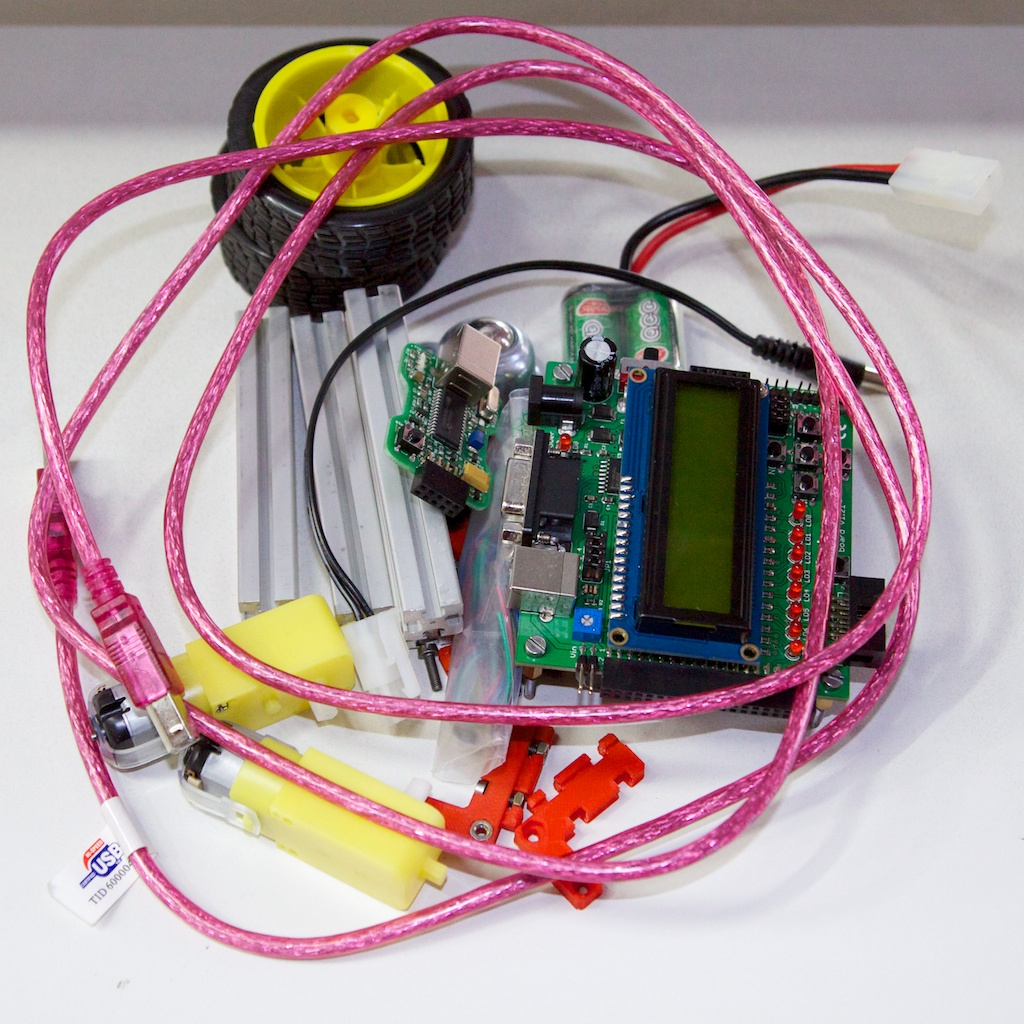
\includegraphics[width=0.5\textwidth]{img/robot_parts.jpg}\label{fig:parts}
\caption[]{Parts}
\end{center}
\end{figure}

\section{Inquiry based robotics learning}
Details of the setup of the workshops itself, all pedagogical aspects.

\begin{figure}[htp]
\subfigure[]{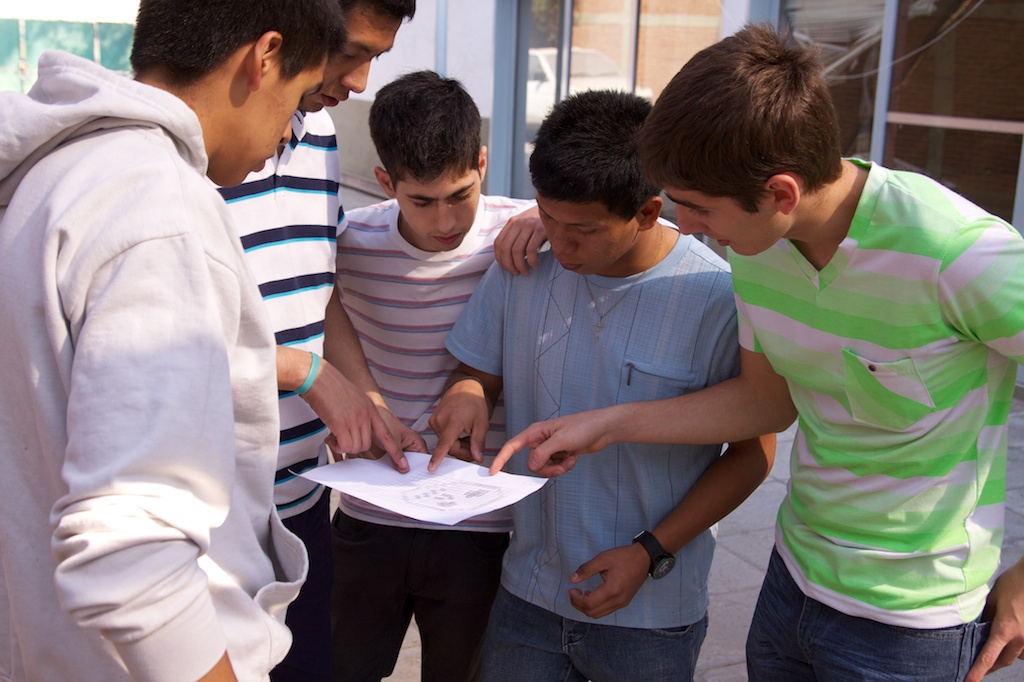
\includegraphics[width=0.325\textwidth]{img/cs_unplugged.jpg}\label{fig:cs_unplugged}}
\subfigure[]{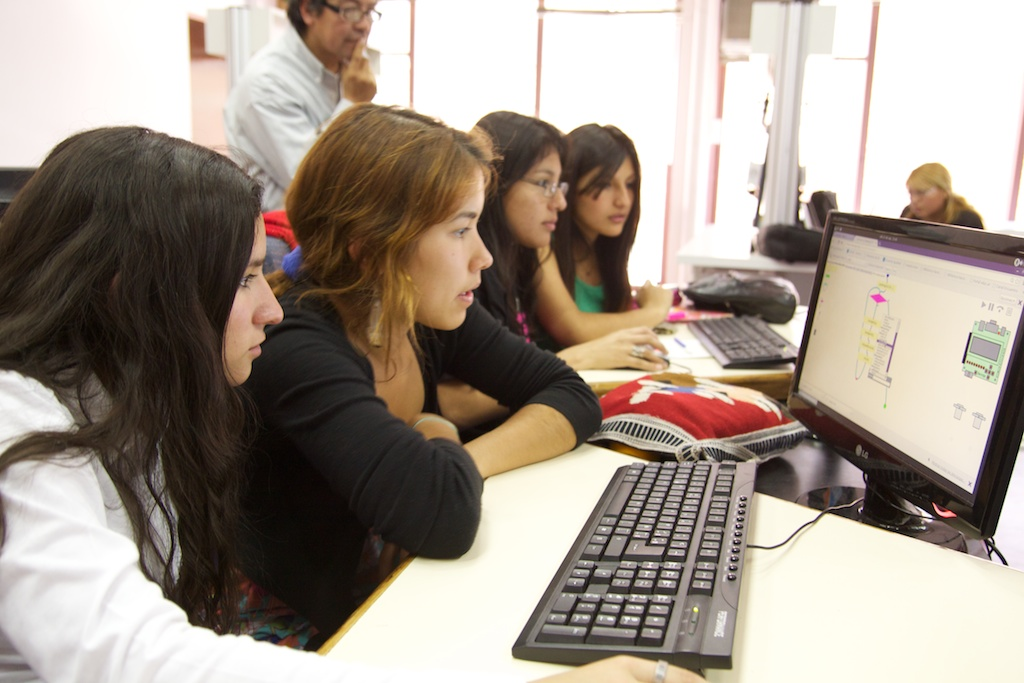
\includegraphics[width=0.325\textwidth]{img/programming.jpg}\label{fig:programming}}
\subfigure[]{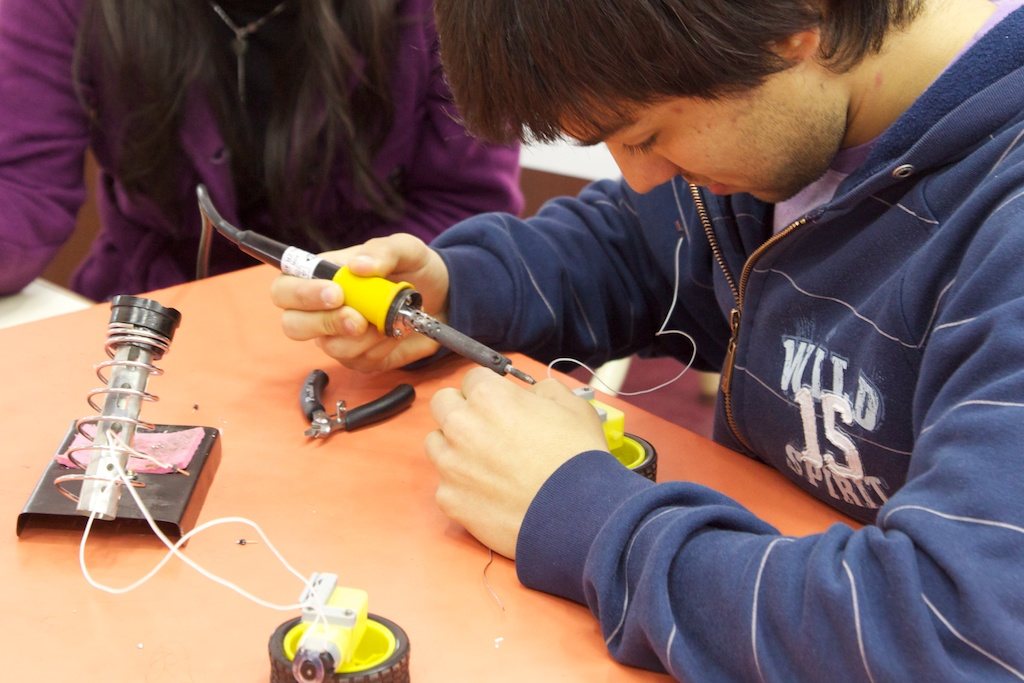
\includegraphics[width=0.325\textwidth]{img/robot_soldering.jpg}\label{fig:soldering}}
\subfigure[]{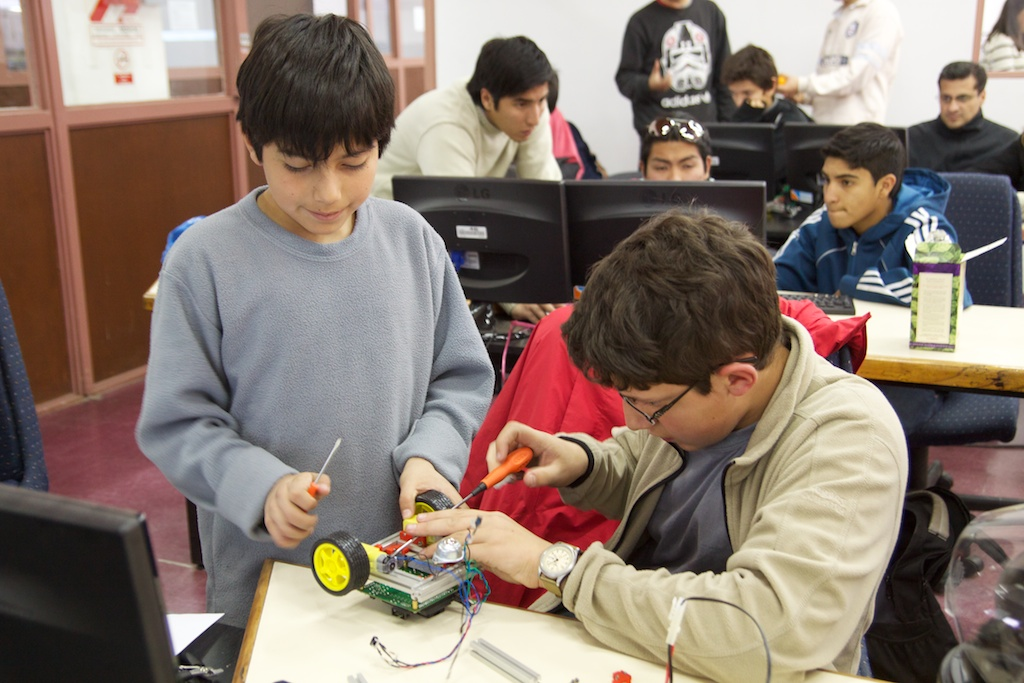
\includegraphics[width=0.325\textwidth]{img/robot_building_a.jpg}\label{fig:building_a}}
\subfigure[]{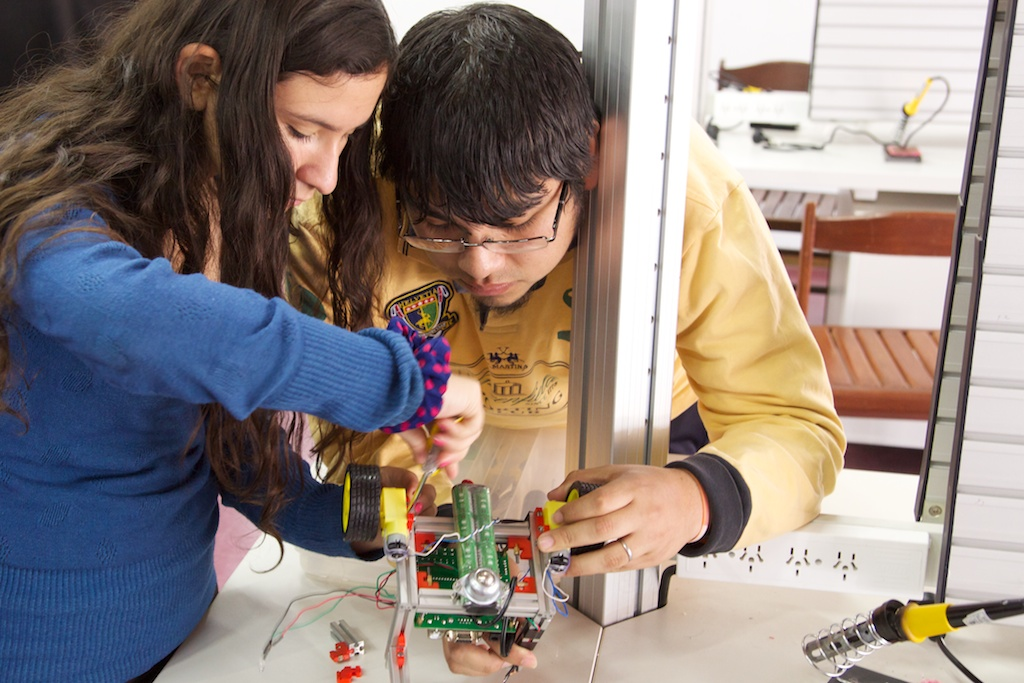
\includegraphics[width=0.325\textwidth]{img/robot_building_b.jpg}\label{fig:building_b}}
\subfigure[]{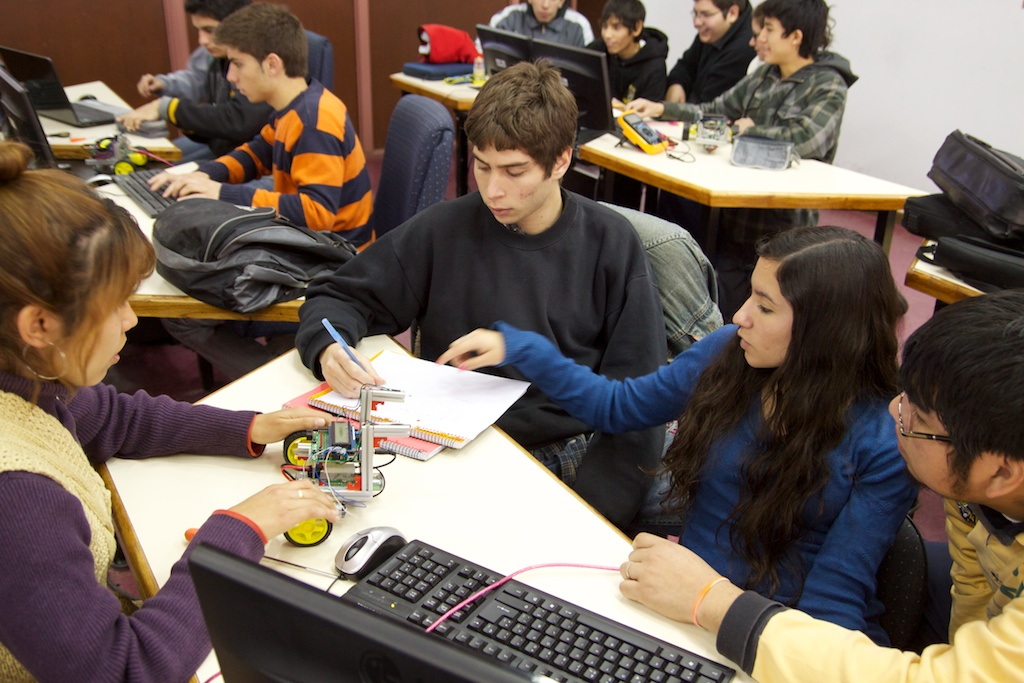
\includegraphics[width=0.325\textwidth]{img/robot_programming.jpg}\label{fig:robot_programming}}
\subfigure[]{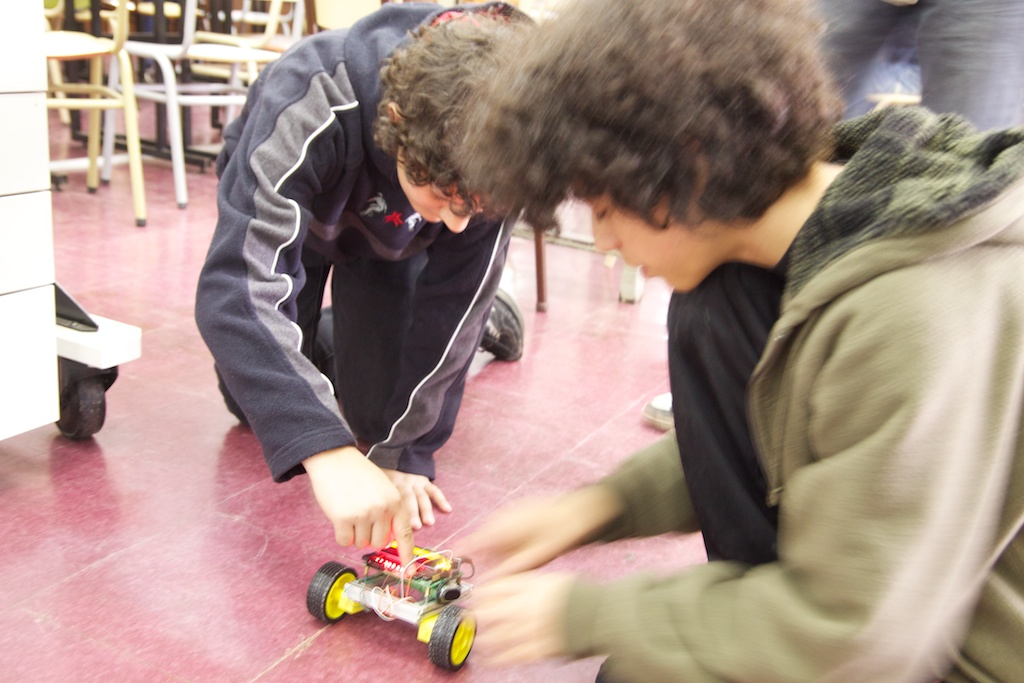
\includegraphics[width=0.325\textwidth]{img/robot_testing_a.jpg}\label{fig:robot_testing_a}}
\subfigure[]{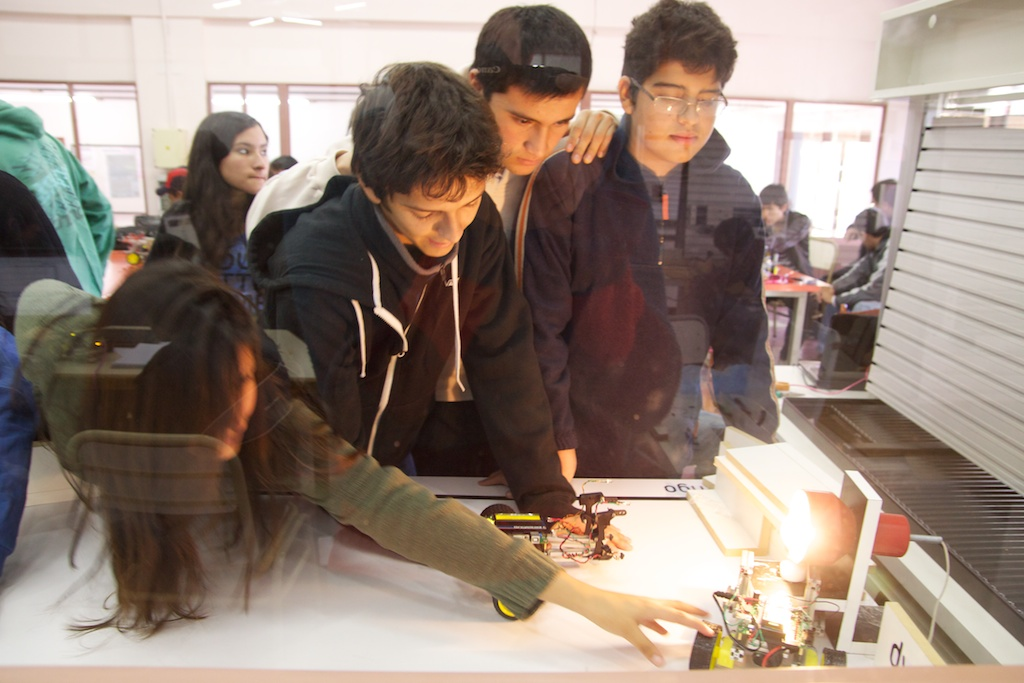
\includegraphics[width=0.325\textwidth]{img/robot_testing_b.jpg}\label{fig:robot_testing_b}}
\subfigure[]{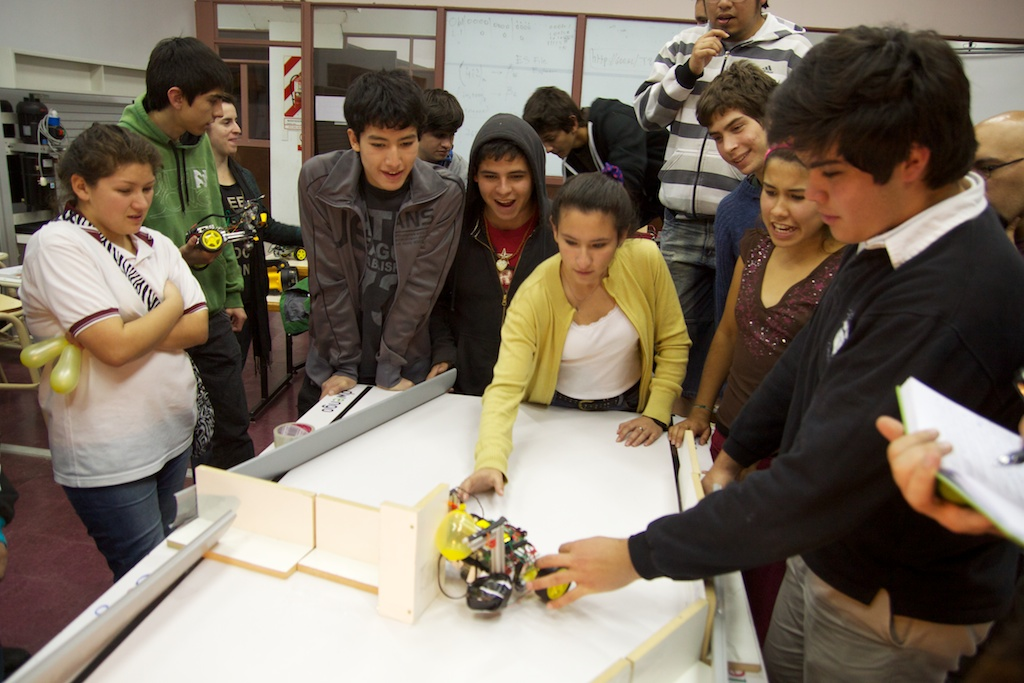
\includegraphics[width=0.325\textwidth]{img/competition.jpg}\label{fig:competition}}
\caption[]{Robotics workshop outline: (a) introduction to the main concepts of computer science by CS Unplugged based games; (b) learning the basics of programming in a graphical programming language; (c) soldering the electronics parts; (d) and (e) building the robot; (f) designing and implementing a strategy to solve task; (g) and (h) testing and improving the robot in a real world setting; (i) the moment of truth, the robot competition.}
\end{figure}

\section{Robotics trick students into learning}
Robots build by the students, details of the google blockly results (for example, one student, aged 13 was able to complete all 10 mazes within xx minutes while others including teachers took 2 hours), feedback given by students and teachers and the scores given.

\section{From a local project to international outreach}
Direct impact: amount of students and teachers we taught, parents that came and visited the competitions, media attention in Salta; Sustainability of the impact: local production of the Dwengo board, continuation of the project in the schools (driven by a careful selection of the teachers and continuous stimulation of them), and the outreach to other countries including Brazils and Bolivia? Chile?

\section{Conclusions}
Goals that we met, collaboration on an international level, decentralisation, spread of pedagogical ideas, technology and values.


%%%%%%%%%%%%%%%%%%%%%%%%%%%%%%%%%%%%%%%%%%%%%%%%%%%%%%%%%%%%%%%%%%%%%%%%%%%%%%%%
\section*{Acknowledgment}
The project presented in this paper was never possible without the unconditional support of the Dwengo volunteers, the newly designed building bricks for robots by Cesar Vandevelde of the Howest, the financial support by Google within the Google RISE framework, the corporation of Dra. Mar\'ia Soledad Vicente of Ministry of Education, Science and Technology of the Salta province, and the infrastructure and support of the U.F.I.De.T.

%%%%%%%%%%%%%%%%%%%%%%%%%%%%%%%%%%%%%%%%%%%%%%%%%%%%%%%%%%%%%%%%%%%%%%%%%%%%%%%%
\bibliographystyle{IEEEtran}
\bibliography{trtwr2014}

\end{document}
